\section{Eletrização por contato e por indução}

\frame{
	\frametitle{Princípio da conservação das cargas}
	\begin{block}{Definição}
		O princípio da conservação da carga elétrica afirma que a soma algébrica das cargas antes e depois de um processo de transferência \textbf{deve ser a mesma}. Assim, podemos dizer que a carga elétrica não pode ser criada nem destruída, somente \textbf{transferida entre corpos}.
	\end{block}
}

\frame{
	\frametitle{Princípio da conservação das cargas}
	\begin{block}{Exemplo}
		Imagine o processo de eletrização por atrito. Inicialmente os corpos a serem friccionados estão neutros, ou seja, apresentam o mesmo número de elétrons e prótons. Após o atrito, um dos corpos cede elétrons e torna-se positivamente eletrizado. O outro  recebe os elétrons, tornando-se negativamente eletrizado. Pela conservação da carga elétrica, podemos dizer que o número de elétrons em excesso em um dos corpos é exatamente igual ao número de prótons em excesso no outro. \textbf{Houve apenas transferência de carga elétrica}.
		\begin{itemize}
			\item A mesma observação pode ser feita a respeito dos processos de eletrização por contato e indução.
		\end{itemize}
	\end{block}
}

\frame{
	\frametitle{Múltiplos e submúltiplos}
	
	\begin{minipage}{0.49\linewidth}
		\resizebox{\textwidth}{!}{
			\begin{tabular}{lcc}
				\toprule
				Prefixo & Símbolo & Expoente \\\midrule
				yocto 	& y & -24\\
				zepto 	& z & -21\\
				atto 	& a &-18\\
				femto 	& f & -15\\
				pico 	& p &-12\\
				nano 	& n &-9\\ 
				micro 	& µ & -6\\
				milli 	& m & -3\\	
				centi 	& c & -2\\	
				deci 	& d &-1\\\bottomrule 
		\end{tabular}}
	\end{minipage}
	\hfill
	\begin{minipage}{0.49\linewidth}
		\resizebox{\textwidth}{!}{
			\begin{tabular}{lcc}
				\toprule
				Prefixo & Símbolo & Expoente \\\midrule
				deca 	& da & 1\\
				hecto 	& h & 2\\
				kilo 	& k & 3\\
				mega 	& M & 6\\
				giga 	& G & 9\\
				tera 	& T & 12\\
				peta 	& P & 15\\
				exa		& E & 18\\
				zetta	& Z & 21\\
				yotta	& Y & 24\\\bottomrule
		\end{tabular}}
	\end{minipage}
	
%	\centerline{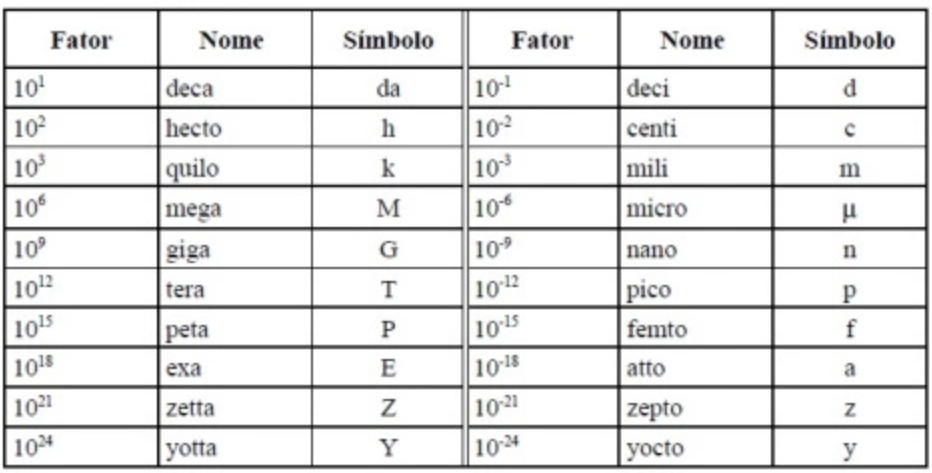
\includegraphics[width=1.05\linewidth]{Figuras/Ch04/multiplos.PNG}}
}

\frame{
	\frametitle{Eletrização por contato}
	\begin{block}{Definição}
		Se dois corpos condutores, sendo pelo menos um deles eletrizado, são postos em contato, a carga elétrica tende a se estabilizar, sendo redistribuída entre os dois, fazendo com que \textbf{ambos tenham a mesma carga}, inclusive com \textbf{mesmo sinal}.
	\end{block}
}

\frame{
	\frametitle{Eletrização por contato}
	\centerline{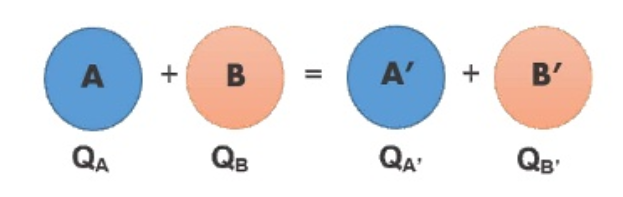
\includegraphics[width=0.7\linewidth]{Figuras/Ch04/conservacao.PNG}}
	\vspace{0.2cm}
	$$\boxed{Q_A + Q_B = Q_{A'} + Q_{B'}}$$
}

\frame{
	\frametitle{Eletrização por contato}
	\begin{block}{O processo - antes}
		\begin{itemize}
			\item O corpo eletrizado transfere cargas elétricas ao corpo neutro, o que ocorre devido à força natural da distribuição de cargas elétricas por dois ou mais materiais condutores.
		\end{itemize}
	\end{block}
	\centerline{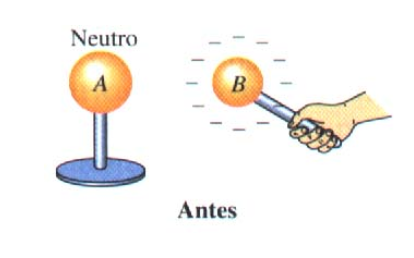
\includegraphics[width=0.6\linewidth]{Figuras/Ch04/antes.PNG}}
}

\frame{
	\frametitle{Eletrização por contato}
	\begin{block}{O processo - durante}
		\begin{itemize}
			\item As cargas em excesso do condutor eletrizado negativamente se repelem e alguns elétrons passam para o corpo neutro, fazendo com que ele fique também com elétrons em excesso e, portanto, eletrizado negativamente.
		\end{itemize}
	\end{block}
	\centerline{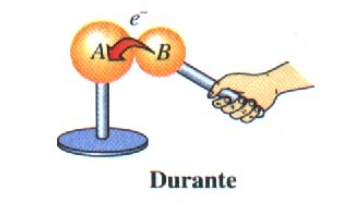
\includegraphics[width=0.55\linewidth]{Figuras/Ch04/durante.PNG}}
}

\frame{
	\frametitle{Eletrização por contato}
	\begin{block}{O processo - depois}
		\begin{itemize}
			\item Os corpos condutores ficam eletrizados com cargas de mesmo sinal, e não necessariamente em mesma intensidade.
		\end{itemize}
	\end{block}
	\centerline{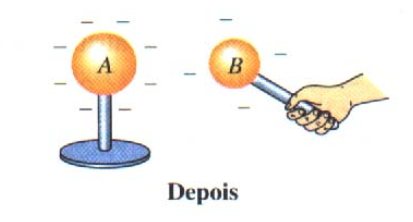
\includegraphics[width=0.6\linewidth]{Figuras/Ch04/depois.PNG}}
}

\frame{
	\frametitle{Eletrização por contato}
	\begin{block}{Cálculo}
		\begin{itemize}
			\item A troca das cargas depende das dimensões dos condutores.
			\item Se considerarmos que os corpos têm as \textbf{mesmas dimensões e a mesma forma}, sendo, por exemplo, esferas de mesmo raio, \textbf{após o contato apresentarão cargas iguais}.
		\end{itemize}
	
		\vspace{0.2cm}
		$$\boxed{Q' = Q_{A'} = Q_{B'} = \dfrac{Q_A + Q_B}{2}}$$
	\end{block}

}

\frame{
	\frametitle{Eletrização por contato}
	\begin{block}{Exemplo \#01}
		Um corpo condutor A com carga $Q_1 = +\SI{6}{\coulomb} $ é posto em contato com outro corpo neutro $Q_N = \SI{0}{\coulomb} $. Qual é a carga em cada um deles após serem separados?
	\end{block}
}

\frame{
	\frametitle{Eletrização por contato}
	\begin{block}{Resolução}
		\[ Q' = Q_{1'} = Q_{N'} = \dfrac{Q_1 + Q_N}{2} = \dfrac{+6 + 0}{2} = +\SI{3}{\coulomb} \]
	\end{block}
}

\frame{
	\frametitle{Eletrização por contato}
	\begin{block}{Exemplo \#02}
		Um corpo condutor A com carga $Q_A = \SI{-1}{\coulomb} $ é posto em contato com outro corpo condutor B com carga $Q_B = \SI{-3}{\coulomb} $. Após serem separados os dois corpos, o corpo A é posto em contato com um terceiro corpo condutor C de carga $Q_C = +\SI{4}{\coulomb} $. Qual é a carga em cada um após serem separados?
	\end{block}
}

\frame{
	\frametitle{Eletrização por contato}
	\begin{block}{Resolução}
		Para o primeiro contato:
		$$Q' = Q_{A'} = Q_{B'} = \dfrac{Q_A + Q_B}{2} = \dfrac{-1 + (-3)}{2} = \SI{-2}{\coulomb} $$
		
		Para o segundo contato:
		$$Q'' = Q_{A''} = Q_{C''} = \dfrac{Q_A' + Q_C}{2} = \dfrac{-2 + 4}{2} = +\SI{1}{\coulomb} $$
		
		Logo, corpo A possui $+\SI{1}{\coulomb}$, corpo B possui \SI{-2}{\coulomb}, e o corpo C possui $+\SI{1}{\coulomb}$.
	\end{block}
}

\frame{
	\frametitle{Eletrização por contato}
	\begin{block}{E se forem raios diferentes?}
		(UTFPR) Uma esfera metálica A de raio de \SI{20}{\centi\meter} está eletrizada com carga $Q$. Essa esfera é conectada com outra esfera B, depois é desconectada de B e conectada com outra esfera C sendo ainda desconectada de C e conectada com uma esfera D. As esferas B, C e D têm raios de \SI{10}{\centi\meter}, também são metálicas (condutoras) e estavam inicialmente neutras. Verifica-se que a esfera D adquire carga elétrica igual a \SI{4}{\micro\coulomb}. Qual a carga elétrica inicial $Q$, da esfera maior?
	\end{block}
}

\frame{
	\frametitle{Eletrização por contato}
	\begin{block}{Resolução}
		Quando os raios são diferentes o maior fica com mais carga, e a carga é proporcional ao raio -- como o corpo A tem o dobro do raio, ele tem que ficar com o dobro da carga.
		
		\vspace{0.2cm}
		
		Como o corpo A tinha carga $Q$ e o corpo B tinha carga zero no começo, a carga total é $Q$, que deverá permanecer a mesma no final (conservação das cargas).
	\end{block}
}

\frame{
	\frametitle{Eletrização por contato}
	\begin{block}{Resolução}
		Se o corpo B ficar com carga $X$ a carga do A tem que ser $2X$, então $X + 2X = Q$.
		
		\vspace{0.2cm}
		
		Logo, o corpo B fica com carga $Q/3$ e o corpo A com carga $2X = 2Q/3$.
		
		\vspace{0.2cm}
		
		Em seguida o corpo A vai ser colocado em contato com o C. Agora pode-se fazer o mesmo procedimento, começando com o corpo A tendo carga $2Q/3$ e o C carga nula e descobrir a carga final de cada um. Repetir o processo até o final. \alert{Terminar de resolver na lista de exercícios 04!!}
	\end{block}
}

\frame{
	\frametitle{Eletrização por indução eletrostática}
	\begin{block}{Definição}
		Este processo de eletrização é totalmente baseado no \textbf{princípio da atração e repulsão}, já que a eletrização ocorre apenas com a aproximação de um corpo eletrizado (indutor) a um corpo neutro (induzido).
	\end{block}
}

\frame{
	\frametitle{Eletrização por indução eletrostática}
	\begin{block}{Etapas}
		\begin{enumerate}
			\item Primeiramente um bastão eletrizado é aproximado de um condutor inicialmente neutro. Pelo princípio de atração e repulsão, os elétrons livres do induzido são atraídos/repelidos dependendo do sinal da carga do indutor.
		\end{enumerate}
	\end{block}

	\centerline{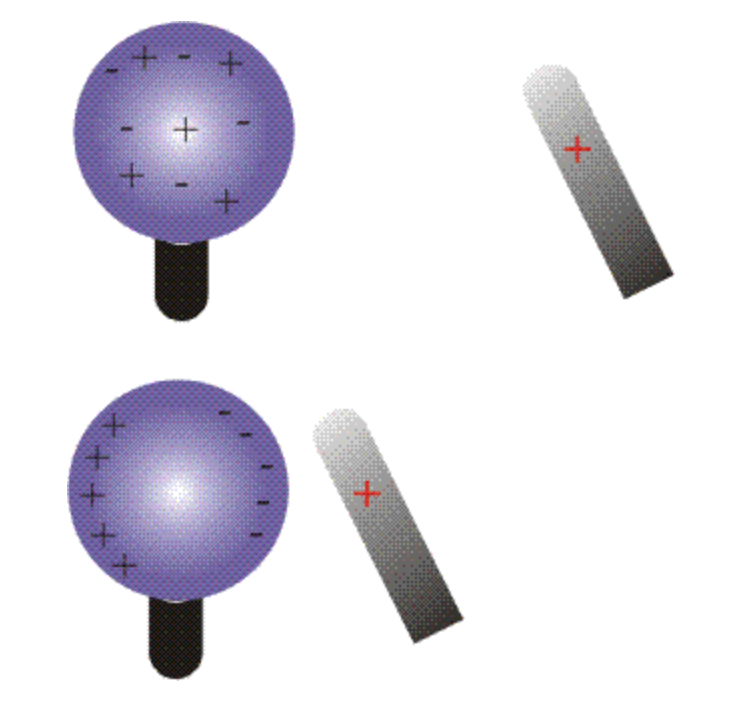
\includegraphics[width=0.45\linewidth]{Figuras/Ch04/inducao1.PNG}}
}

\frame{
	\frametitle{Eletrização por indução eletrostática}
	\begin{block}{Etapas}
		\begin{enumerate}
			\setcounter{enumi}{1}
			\item O próximo passo é ligar o induzido à terra, ainda na presença do indutor. Os elétrons da terra são conduzidos pelo fio condutor para a parte positiva da esfera no sentido de neutralizá-la.
		\end{enumerate}
	\end{block}

	\centerline{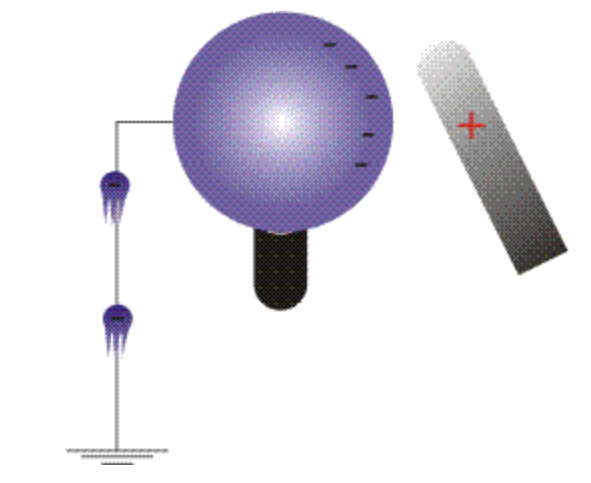
\includegraphics[width=0.45\linewidth]{Figuras/Ch04/inducao2.PNG}}
}

\frame{
	\frametitle{Eletrização por indução eletrostática}
	\begin{block}{Etapas}
		\begin{enumerate}
			\setcounter{enumi}{2}
			\item Desliga-se o induzido da terra. Pode-se retirar o indutor das proximidades e o induzido estará eletrizado com sinal oposto à carga do indutor e as cargas se distribuem por todo o corpo.
		\end{enumerate}
	\end{block}

	\centerline{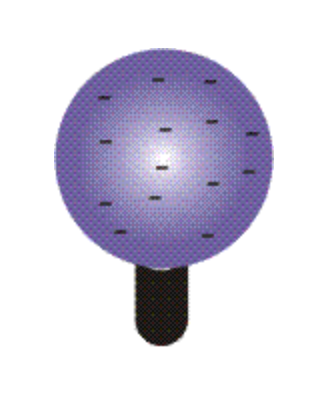
\includegraphics[width=0.35\linewidth]{Figuras/Ch04/inducao3.PNG}}
}

\frame{
	\frametitle{Eletrização por indução eletrostática}
	\begin{block}{Na natureza}
		Um exemplo de uma consequência da eletrização por indução são os raios. Quando temos uma nuvem carregada eletricamente durante uma tempestade, ela irá induzir na superfície cargas de sinais opostos criando assim um campo elétrico entre a nuvem e a superfície. Se esse campo elétrico for muito intenso teremos uma descarga elétrica violenta que nós conhecemos como raio.
	\end{block}

	\centerline{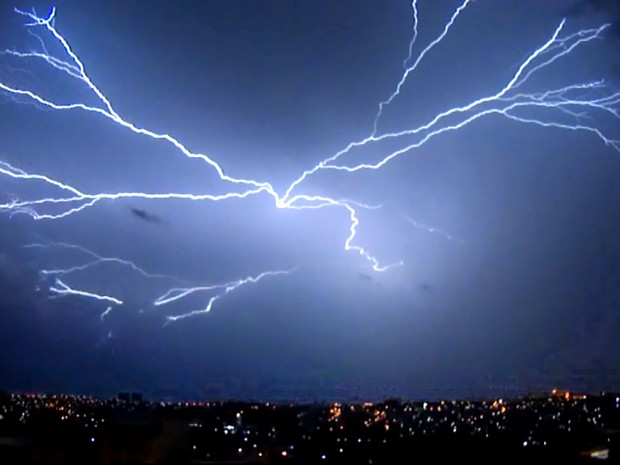
\includegraphics[width=0.4\linewidth]{Figuras/Ch04/raios.jpg}}
}

\section*{Exercícios}

\frame{
	\frametitle{Exercícios}
	\begin{block}{}
		01. Quatro corpos, A, B, C e D formam um sistema eletricamente isolado. Inicialmente tem-se que $Q_A = \SI{6}{\micro\coulomb} $, $Q_B = \SI{-2}{\micro\coulomb} $, $Q_C = \SI{4}{\micro\coulomb} $ e $Q_D = \SI{-4}{\micro\coulomb} $. O corpo A cede $\SI{2}{\micro\coulomb} $ ao corpo B e o corpo C cede $ \SI{1}{\micro\coulomb} $ ao corpo D. Assinale a afirmação incorreta:\\

		\vspace{0.5cm}

		(a) O corpo B ficou eletricamente neutro. \\

		\vspace{0.3cm}

		(b) A carga total após a transferência é de \SI{4}{\micro\coulomb}. \\

		\vspace{0.3cm}

		(c) A soma algébrica das quantidades de carga elétrica é constante. \\

		\vspace{0.3cm}

		(d) O corpo A, antes e depois, tem carga elétrica positiva. \\

		\vspace{0.3cm}

		(e) Após a transferência de carga os corpos C e D ficaram eletricamente positivos.
	\end{block}
}

\section*{Referências}

\frame{
	\frametitle{Referências e Exercícios Complementares}
	\begin{itemize}
		\item Física, Ciência e Tecnologia – Vol 3. PENTEADO, Paulo César M; TORRES, Carlos Magno A. Ed. Moderna (2006)
	\end{itemize}
	%\centering{\alert{Página 36 - \textbf{1.6.1 até 1.6.5, 1.6.17 até 1.6.19}}} \\
	%https://www.youtube.com/watch?v=IUgS7Uw-qBI
	\centering{\alert{Lista de exercícios 04}}
}